\documentclass[11pt,a4paper]{letter}
\usepackage[top=1.00in, bottom=1.0in, left=.75in, right=0.75in]{geometry}
\usepackage{graphicx}
\usepackage{natbib}

\address{1300 Centre Street \\ Boston, MA, 20131}

\begin{document}
\bibliographystyle{..//..//refs/bibstyles/amnat.bst}
\begin{letter}{}
\includegraphics[width=0.5\textwidth]{/Users/aileneettinger/Dropbox/Documents/Work/AA_heading.pdf}
\pagenumbering{gobble}

\opening{Dear Dr. ??:}
We propose a ``Perspective" on implications of the altered photoperiod that organisms will experience due to climate change-induced spatial and temporal shifts. 
We believe this piece would be of broad interest to readers of \emph{Nature Climate Change}. Photoperiod acts as a cue for responses such as spring emergence and migration timing for diverse species, and alterations to experienced photoperiod may therefore affect development, growth, and fitness for plants, insects, fish, and mammals, among other organisms. Yet, photoperiod has rarely been included in forecasts of species responses to climate change and implications of climate change induced shifts in photoperiod are largely unexplored, especially for early-season spring events. 
\\
\\
With recent climate change, species have moved in space (altitudinal and latitudinal range shifts) and in time (phenological shifts) (Chen et al 2011,Parmesan and Yoke 2003) and both types of shifts result in altered photoperiod regimes (Saikkonen et al 2012).  Altered photoperiods have the potential to dramatically alter species' performance and fitness, since daylength can affect the timing of development, migration, and other critical responses.  However, the magnitude of effects of shifts in photoperiod with climate change are unknown or unquantified for the vast majority of species.  Our Perspective would quantify expected changes in experienced photoperiod due to shifts in space versus in time, given observations to date (e.g., Chen et al 2011, Parmesan and Yoke 2003), and put them in a novel, global context. For example, previous work has focused on effects geographic shifts in species distributions on photoperiod (e,g,, Saikkonen et al 2012, Way and Montgomery 2015). We would demonstrate that impacts on experienced photoperiod due to temporal shifts will be orders of magnitude larger than impacts due to spatial shifts (e.g., 1.6 hours of change versus one minute of change). 
\\
\\
Our ``Perspective" would also offer a valuable addition to current approaches because it would focus on spring phenology events. To date, the role of photoperiod has received far more detailed attention for end-of-season activities such as growth cessation in the fall than for spring. Understanding the role of photoperiod in spring events  is critical in the context of a changing climate because phenology during this season is currently responding strongly to shifts in temperature. If photoperiod limitations come into play, however, the rapidly advancing springs may abruptly cease advancement. We will demonstrate that incorporating photoperiod into forecasts may be possible for some species by leveraging existing experimental data (cite ospree database). For example, growth chamber experiments on woody plant spring phenology often have data relevant for climate change impacts. We plan to highlight how new modelling approaches to improve predictions of when, where, and how much photoperiod is likely to affect future spring phenology could be combined with new empirical work to improve our understanding of the role of photoperiod in a warming world (Figure 1).
\\
We expect the title of our manuscript to be ``Spatial and temporal shifts in photoperiod with climate change."  Thank you for considering our paper.

Sincerely,\\

\includegraphics[scale=1]{/Users/aileneettinger/Dropbox/Documents/Work/AileneEttingerSignature.png} \\
Ailene Ettinger
NRC Research Assocaite, Northwest Fisheries Science Center

\noindent \emph{References mentioned in cover letter}
\begin{footnotesize}
\begin{enumerate}
\item Chen, I.-C., J. K. Hill, R. Ohlemueller, D. B. Roy, and C. D. Thomas. 2011. Rapid range shifts of species associated with high levels of climate warming. Science 333:1024{1026.

\item Saikkonen, K., K. Taulavuori, T. Hyvonen, P. E. Gundel, C. E. Hamilton, I. Vanninen, A. Nissinen, and M. Helander. 2012. Climate change-driven species' range shifts filtered by photoperiodism. \emph{Nature Climate Change} 2:239.

\item Way, D. A., and R. A. Montgomery. 2015. Photoperiod constraints on tree phenology, performance and migration in a warming world. \emph{Plant, Cell \& Environment}38:1725-1736.

\end{enumerate}
\end{footnotesize}

\begin{figure}[p]

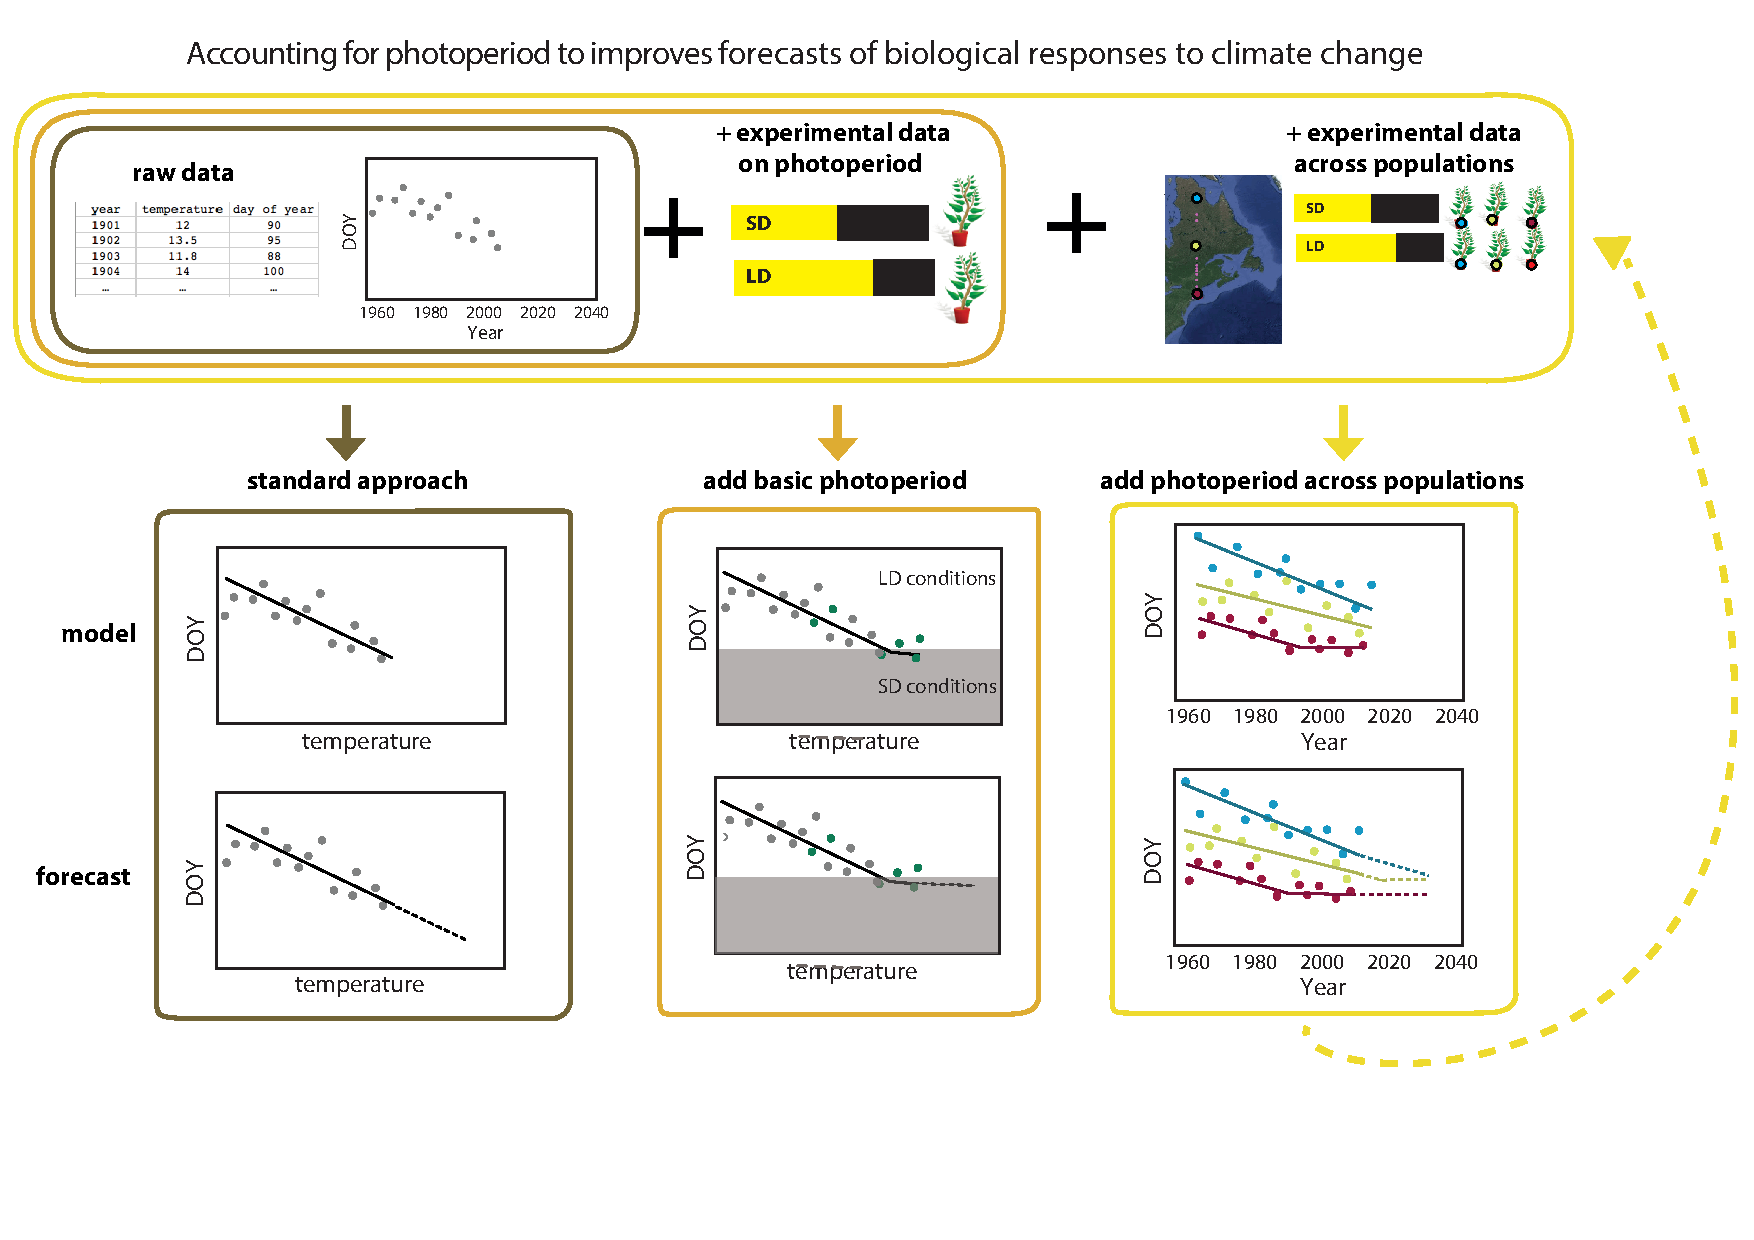
\includegraphics[width=180mm,scale=0.5]{..//..//analyses/photoperiod/figures/photocondiag6.pdf} 
\caption{\textbf{Conceptual diagram of how to include photoperiod in forecasting biological responses to climate change}. Current approaches for forecasting spring phenology with climate change frequently rely on linear relationships between historical temperature data and observed dates of spring phenology (left panels). Adding responses to photoperiod, which commonly operate as threshold responses to short days (SD) versus long days (LD), will alter these forecasts (center panel) in ways that differ across species that differ in their respective threshold photoperiods. Other factors that interact with photoperiod, such as population-level variation  in photoperiod responses, can be incorporated into forecasts to further improve their accuracy (right panel).}
 \label{fig:condiag}
 \end{figure}

\end{letter}
\end{document}
